\documentclass[12pt, a4paper]{report}

\usepackage[utf8]{inputenc}
\usepackage{amsfonts, amssymb, amsmath}
\usepackage{csquotes}
\usepackage[english]{babel}
\usepackage{newlfont}
\usepackage{color}
\textwidth=450pt\oddsidemargin=0pt
\usepackage[top=3cm, bottom=3.5cm,left=2.5cm, right=2.5cm]{geometry}
\usepackage{graphicx}
\usepackage{float}
\usepackage{comment}
\usepackage{caption}
\usepackage{subcaption}
%\usepackage[labelformat=empty]{caption}
\usepackage{float}
\usepackage[separate-uncertainty=true]{siunitx}
\usepackage[style=numeric,backend=biber, sorting=none]{biblatex}
\usepackage{titlesec}
\usepackage{dsfont}
\usepackage{listings}
\usepackage[colorlinks=true, linkcolor=blue, urlcolor=cyan, citecolor=green]{hyperref}
\usepackage{cleveref}
\usepackage{xcolor}
\usepackage{xparse}
\usepackage{siunitx}

\addbibresource{thesis.bib}

\numberwithin{equation}{section}

\parindent=0pt

\title{Thesis}
\author{Samuele De Amicis}

\begin{document}

\maketitle

\chapter{Froehlich Polaron}
\section{Electrons in crystals}
The study of electrons inside a solid crystal is an important field due to their role in the determination of transport
and optical properties of such materials.\\
Multiple experiments involving X-ray or electron scattering from suitable solid samples have demonstrated that a crystalline solid, 
whether a metal, an insulator or a semiconductor, is described a periodic arrangement of atoms consisting of a unit cell 
(usually the primitive one, defined as the smallest unit cell possible in a determined material) with a suitable 
atomic basis: some examples are Iron (Fe), described by a BCC (Body-Centered Cubic) unit cell with a single Fe atom basis, 
rock salt (NaCl), described by by a FCC (Face-Centered Cubic) unit cell with a basis composed of one Na atom and one Cl atom, and 
crystalline silicon (Si), which is characterized by the diamond structure, an FCC structure with a basis composed of 2 silicon atoms 
(geometrically different from that seen in rock salt). \\
Given the periodic nature of crystal structures, it is natural to consider the electrostatic potential generated by the crystal to 
be periodic too. Such is the basic assumption which underlies the treatment of electrons in crystals, that was first described by 
Felix Bloch in his famous 1928 paper \textit{Uber die Quantenmechanikder Elektronen in Kristallgittern} \cite{bloch1928quantum}.\\
The model proposed by Bloch assumed independent electrons (no electron-electron interactions terms): each electron behaves as 
if only an average contribution to the potential from the other electrons (with the same periodicity of the lattice) exists, thus 
retrieving an \textbf{effective one-electron potential}.\\
The resulting Hamiltonian for the single independent electron is:
\begin{equation}
    \mathrm{H}\psi(\mathbf{r})=\left(-\frac{\hbar^2}{2m}\nabla^2+V(\mathbf{r})\right)\psi(\mathbf{r})=E\psi(\mathbf{r}),
    \label{eq_0_00}
\end{equation}
where $V(r)$ is a periodic potential with the lattice periodicity, given a lattice translation vector
\begin{equation}
    \mathbf{T}=n_1\mathbf{a}_1+n_2\mathbf{a}_2+n_3\mathbf{a}_3,\hspace{1cm}n_1,n_2,n_3\hspace{0.5cm}\mathrm{integers},
\end{equation}
with $\mathbf{a}_1$, $\mathbf{a}_2$ and $\mathbf{a}_3$ primitive translation vectors.
Therefore, we have
\begin{equation}
    V(\mathbf{r}+\mathbf{T})=V(\mathbf{r})
\end{equation}
This means that the potential can be expanded in Fourier series
\begin{equation}
    V(\mathbf{K})=\sum_\mathbf{K}V_\mathbf{K}e^{i\mathbf{K}\cdot \mathbf{r}},
\end{equation}
and is consequently useful to expand the wavefunction in the same way. For this reason the Born-von Karman boundary conditions
are applied \cite{Ashcroft76}
\begin{equation}
    \psi(\mathbf{r}+N_i\mathbf{a}_i)=\psi(\mathbf{r}),\hspace{1cm}i=1,2,3.
\end{equation}
where $N_i\mathbf{a}_i$ is a chosen vector such that $V(r+N_ia_i)=V(\mathbf{r})$ (it is a translation vector for the lattice). This is a normalizing
condition for the wavefunction which corresponds to taking $N_i$ unit cell in each direction and periodically repeating them. In this 
way it is possible to write the wavefunction in the following way:
\begin{equation}
    \psi(\mathbf{r})=\sum_\mathbf{q}c_\mathbf{q}e^{i\mathbf{q}\cdot\mathbf{r}}.
    \label{eq_0_01}
\end{equation}
Going back to the periodic potential $U(\mathbf{r})$ we observe that the Fourier terms $U_\mathbf{K}$ are related to $U(\mathbf{r})$ by
\begin{equation}
    U_\mathbf{K}=\frac{1}{V}\int_{cell}dre^{-i\mathbf{K}\cdot\mathbf{r}}U(\mathbf{r})
\end{equation}
with $V$ unit cell volume and $\mathbf{K}$ reciprocal lattice vector (vector in k-space such that $e^{i\mathbf{K}\cdot \mathbf{a}_i}=1$). If it is 
assumed that the potential $V(\mathbf{r})$ is real and $V(-\mathbf{r})=V(\mathbf{r})$ (valid for every Bravais lattice) it follows that the coefficients 
$U_\mathbf{K}$ are real.\\
Substituting in \ref{eq_0_00} we obtain:
\begin{equation}
    (\mathrm{H}-E)\psi(\mathbf{r})=\sum_\mathbf{q}\left(\frac{\hbar^2}{2m}q^2-E\right)c_\mathbf{q}e^{i\mathbf{q}\cdot\mathbf{r}}+\sum_{\mathbf{K}\mathbf{q}'}U_\mathbf{K}c_{\mathbf{q}'-\mathbf{K}}e^{i\mathbf{q}'\cdot\mathbf{r}}=0,
\end{equation}
which yields the following result:
\begin{equation}
    \left(\frac{\hbar^2}{2m}(\mathbf{k}-\mathbf{K})^2-E\right)c_{\mathbf{k}-\mathbf{K}}+\sum_{\mathbf{K}'}c_{\mathbf{K}'-\mathbf{K}}c_{\mathbf{k}-\mathbf{K}'}=0.
\end{equation}
From this equation it becomes clear that for a fixed $k$ only the coefficients $c_\mathbf{k},c_{\mathbf{k}-\mathbf{K}},...$ whose wavevector differs from 
$\mathbf{k}$ by a reciprocal lattice vector are coupled. In this way the original problem has been divided in $N$ independent equations for 
each allowed value of $\mathbf{k}$ (in the first Brillouin zone, the primitive unit cell in the reciprocal space).\\
Going back to the expansion \ref{eq_0_01} the wavefunction now becomes:
\begin{equation}
    \psi_k(r)=\sum_{K}c_{k-K}e^{i(k-K)\cdot r},
\end{equation}
which can be recast as 
\begin{equation}
    \psi_k(r)=e^{ik\cdot r}\sum_{K}c_{k-K}e^{-iK\cdot R};
\end{equation}
in this form it is easy to recognize that 
\begin{equation}
    u_\mathbf{k}(\mathbf{r})=\sum_\mathbf{K}c_{\mathbf{k}-\mathbf{K}}e^{-i\mathbf{K}\cdot\mathbf{R}}
\end{equation}
has the periodicity of the (reciprocal) Bravais lattice.\\
The shape of the Bloch wavefunction as stated in the Bloch theorem is thus retrieved
\begin{equation}
    \psi_\mathbf{k}(\mathbf{r})=e^{i\mathbf{k}\cdot \mathbf{r}}u_\mathbf{k}(\mathbf{r})
\end{equation}
and its square modulus (from which important properties such as charge distribution follow) $|\psi_\mathbf{k}(\mathbf{r})|^2$ has the periodicity of the
lattice.\\
The new Hamiltonian eigenvalues equation using Bloch wavefunction reads
\begin{equation}
    \mathrm{H}_\mathbf{k} u_{n\mathbf{k}}=\left(\frac{\hbar^2}{2m}\left(\frac{1}{i}\nabla+\mathbf{k}\right)^2+U(\mathbf{r})\right)u_{n\mathbf{k}}(\mathbf{r})=E_{n\mathbf{k}}u_{n\mathbf{k}}(\mathbf{r}),
\end{equation}
which yields a different energy eigenvalue for each $\mathbf{k}$ in the first Brillouin zone. The index $n$ arises from the fact that for 
each $\mathbf{k}$ value infinite discrete solutions to the eigenvalue equation exist, in the same as in the particle in a box problem. Going 
to the thermodynamic limit ($N_i\to\infty$ for each component $i$) the entire first Brillouin zone is sampled and the typical band 
structure of the solids is recovered.\\
All the methods employed in solid state calculations rely on this "simple" equation to determine band structures, granted 
analytical form of the periodic potential $U(\mathbf{r})$ can be retrieved.\\
The most used and effective computation method is \textbf{Density Functional Theory} \cite{thijssen2007computational} or \textbf{DFT} 
for short, which does not directly compute the eigenvalue equation for each single $k$ and $n$ value, which would be impossible since 
the potential $U(\mathbf{r})$ is a many-body object that includes electron-electon interactions, but rather computes all the physical quantities of 
interest starting from the ground state charge density $\rho_0(\mathbf{r})$. This is made possible by the two Hohenberg-Kohn theorems \cite{hohenberg1964inhomogeneous}, 
which respectively state that the external potential (the periodic $U(\mathbf{r})$ from the electron point of view) is uniquely determined 
up to a constant by the ground state charge density $\rho_0(\mathbf{r})$ and that this density can be computed variationally by minimizing a suitable 
functional $F[\rho]$.\\
Nevertheless, the functional $F[\rho]$ exact form is unknown: for this reason the \textbf{Kohn-Sham scheme} \cite{PhysRev.140.A1133} 
is used. The idea at the basis of this practical setup is to substitute the real interacting system (many-body) with an auxiliary non-interacting
one (single particle) which has the same ground state as the original. In this system the total potential $V(\mathbf{r})=V_{ion}(\mathbf{r})+V_{ee}(\mathbf{r})$ is 
replaced with an effective potential $V_{eff}(\mathbf{r})$ defined as
\begin{equation}
    U_{eff}(\mathbf{r})=U_{ion}(\mathbf{r})+U_H(\mathbf{r})+U_{xc}(\mathbf{r}),
\end{equation}
where $U_{ion}$ is the ionic potential, often modelled using pseudopotentials \cite{kerker1980non}, $U_H(\mathbf{r})$ is the Hartree term, the electrostatic 
potential due to the mean field distribution of all the other electrons, and $U_{xc}(\mathbf{r})$ the exchange-correlation term, an approximate potential 
which includes Pauli exclusion principle (exchange), higher order electron-electron interactions (correlation) and many body corrections to kinetic energy. The exchange-correlation 
term is usually computed using \textbf{LDA} (Local Density Approximation) or \textbf{GGA} (Generalized Gradient Approximation), both based on the the Uniform Electron 
Gas (UEG) \cite{ziesche1998density}.
Despite the inevitable approximations, DFT calculations are able to provide extremely accurate band structure calculations 
with few drawbacks, such as inaccurate gap estimations in insulators and semiconductors.
\begin{figure}[H]
    \centering
    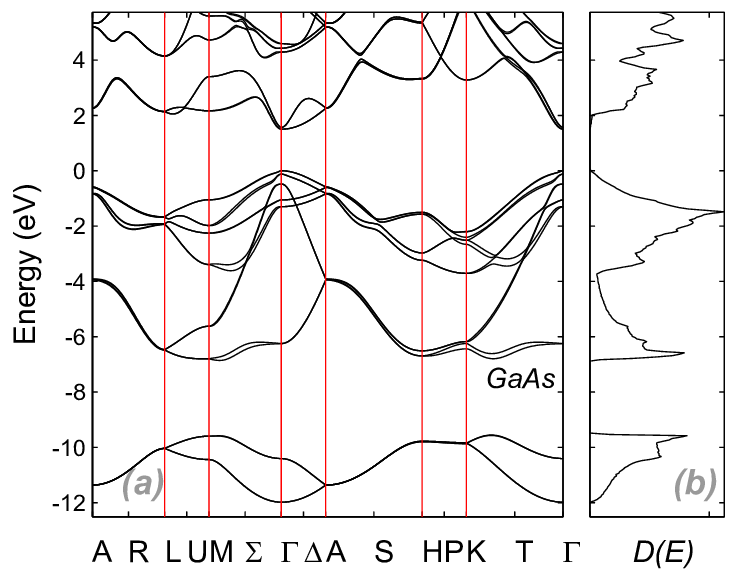
\includegraphics[scale=0.4]{a-Calculated-low-temperature-band-structure-for-GaAs-in-WZ-phase-b-Calculated-DOS.png}
    \caption{DFT calculated low-temperature GaAs Wurtzite structure with relative DOS \cite{GaAs_wurtzite_structure}.}
    \label{fig:GaAs_Wurtzite_structure}
\end{figure}
As it can be seen in Figure \ref{fig:GaAs_Wurtzite_structure} for GaAs, at the band extrema (at the edge between the allowed band states 
and the forbidden gap) the bands have a quadratic dispersion akin to that of a free electron: an electron in these regions only feel a 
very weak external potential $U(\mathbf{r})$ and can be considered as free provided that the free electron mass $m$ is substituted with an effective mass 
$m^*$ which takes into account the potential acting on it.\\
In a general case the effective mass is a tensorial quantity (bands are anisotropic in general with respect to the wavevector) and 
their value can be computed with
\begin{equation}
    m^{*-1}_{ij}=\frac{1}{\hbar^2}\frac{\partial^2 E}{\partial k_i \partial k_j},
    \label{eq_effective_mass}
\end{equation}
provided that the quadratic approximation is valid. This approximation is really useful when calculating quantities near band extrema, 
providing an effective description of an otherwise complex interaction.
\section{The polaron problem: the Froehlich model}
The treatment described up until now for electrons in solids relies on a basic assumption: electro dynamics is much faster than ion 
dynamics. This is the so-called \textbf{Born-Oppenheimer approximation}, which assumes that the motion of the much heavier ions is 
slow compared to the fast dynamics of the electrons (the characteristic time are of the order of $ps$ for ions and $fs$ for 
electrons). As a result, electrons are considered to respond instantaneously to changes in the positions of the ions, allowing 
the separation of electronic and ionic degrees of freedom in the analysis. Given $M$ ions and $n$ electrons the wavefunction 
$\Psi(\mathbf{R}_1,...,\mathbf{R}_M,\mathbf{r}_1,...,\mathbf{r}_n)$ with $\mathbf{R}_\alpha$ ionic positions and $\mathbf{r}_i$ electron positions can be decomposed in the following way:
\begin{equation}
    \Psi(\mathbf{R}_1,...,\mathbf{R}_M,\mathbf{r}_1,...,\mathbf{r}_n)=\chi(\mathbf{R}_1,...,\mathbf{R}_M)\psi(\mathbf{r}_1,...,\mathbf{r}_n),
\end{equation}
and only the electronic wavefunction $\psi(\mathbf{r}_1,...,\mathbf{r}_n)$ is taken into consideration, decoupling ionic degrees of freedom and treating 
ionic potential as a constant energy surface $U_{ion}(\mathbf{r})$.\\
This approximation, although extremely effective in computing electronic bands, fails by design to describe systems where there is a 
strong coupling between electrons and ions (for example electron-phonon interaction).\\
Such is the case of polar crystals: in these materials single electrons at the bottom of the conduction band (or holes at the top of 
the valence band) couple to the strongly polarized ions and distort the unit cell: an electron-phonon interaction is thus present 
in the lattice and the electron properties (such as energy and effective mass) are renormalized due to this coupling \cite{frohlich1954electrons}.\\
The basic assumption of the Froehlich model is that the polaron is "large", namely the characteristic size of the polaron (electron together 
with its phonon cloud) is much larger than the lattice constant $a$. In this way it is possible to ignore the atomic details of the actual 
material and treat it as a uniform dielectric medium.\\
It is assumed that the electron which takes part in the formation of the polaron lies at the bottom of the valence band, in this way it is 
expected to have a quadratic energy dispersion characterized (as already seen in \ref{eq_effective_mass}) by an effective mass
\begin{equation}
    \epsilon(k)=\frac{\hbar^2k^2}{2m^*},
\end{equation}
where the effective mass $m^*$ encapsulates all the interactions due to crystal structure (for a hole polaron the dispersion is similar 
considering a negative effective mass).\\
Given the fact that we are dealing with the large polaron model, it is possible to treat the material as an homogeneous continuum 
which is polarized by the excess charge (the conduction electron). We also assume that the material is isotropic.
Let $\mathbf{P}(\mathbf{r})$ be the electric polarization at the point $\mathbf{r}$, the total electric field is then:
\begin{equation}
\begin{split}
    &\mathbf{D}(\mathbf{r})=\epsilon_0\mathbf{E}(\mathbf{r})+4\pi \mathbf{P}(\mathbf{r}),\\
    &\mathbf{D}(\mathbf{r})=\epsilon \mathbf{E}(\mathbf{r}).
\end{split}
\end{equation} 
The only free charge present in the material is the conduction electron in excess, this means that $\mathbf{D}(\mathbf{r})$ is completely determined by it:
\begin{equation}
\begin{split}
    &D(\mathbf{r},\mathbf{r}_{el})=-\nabla\frac{e}{|\mathbf{r}-\mathbf{r}_{el}|}, \\
    &\nabla\cdot \mathbf{D}(\mathbf{r},\mathbf{r}_{el})=4\pi\delta(\mathbf{r}-\mathbf{r}_{el}),
\end{split}
\end{equation}
with $\mathbf{r}_{el}$ the coordinate of the conduction electron. Developing the equations the following relation is obtained:
\begin{equation}
    4\pi \mathbf{P}(\mathbf{r}) = \left(1-\frac{1}{\epsilon}\right)\mathbf{D}(\mathbf{r}).
\end{equation}
$\mathbf{P}(\mathbf{r})$ is the total polarization, which has the contribution both from electrons and from ionic displacements, since only the second 
contribution is relevant in our treatment, a method to tell apart this two contributions is needed.\\
To obtain this we imagine a system where a field is slowly applied and then rapidly switched off \cite{haken1976quantum}: only 
electrons are able to keep up with the variation of the field. A formula connecting polarization and $\mathbf{D}$ (dropping the $\mathbf{r}$ dependence for simplicity 
since an isotropic and homogeneous medium is assumed) is then retrieved as
\begin{equation}
    4\pi \delta \mathbf{P} = -\left(1-\frac{1}{\epsilon_\infty}\right)\mathbf{D},
\end{equation}
it is then obtained the lattice contribution to the polarization:
\begin{equation}
    4\pi \mathbf{P}_{lat} = 4\pi(\mathbf{P}-\delta \mathbf{P}) = \left(\frac{1}{\epsilon_\infty}-\frac{1}{\epsilon_0}\right)\mathbf{D}.
    \label{eq_polarization_lattice}
\end{equation}
We know consider a model for the polar crystal lattice: we assume it to be constituted of individual oscillating discrete dipoles 
located at fixed sites of the crystal with characteristic frequency $\omega$. The energy of each one of these oscillators is 
\begin{equation}
    \frac{M}{2}(\dot{q}^2+\omega^2q^2).
\end{equation}
The next step is to move from a discrete set of fixed oscillators to a continuum of dipoles: it is assumed that the dipoles are not 
coupled. Defining the effective charge as $e^*$, the following substitution is made:
\begin{equation}
    e^*\mathbf{q}_n\to \mathbf{P}_{lat}(\mathbf{r}),
\end{equation}
which relates the dipole moment to the polarization field. We also write the following relation:
\begin{equation}
    \frac{M}{e^{*2}}=\gamma d^3r,
\end{equation}
where $M=nd^3r$ is the mass density of the medium.\\
It is now possible to define the kinetic and potential energy of the freely oscillating polarization field:
\begin{equation}
\begin{split}
    &T=\int \frac{\gamma}{2}\dot{\mathbf{P}}_{lat}^2(\mathbf{r})d^3r,\\
    &V=\int \frac{\gamma\omega^2}{2}\mathbf{P}_{lat}^2(\mathbf{r})d^3r.
\end{split}
\end{equation}
We identify $\omega$ with the optical phonon frequency $\omega_{LO}$, but the constant $\gamma$ has not yet been given a physical 
definition. For this reason we consider the interaction between electrons and dipole moment, which is given by 
\begin{equation}
    e\frac{\mathbf{r}-\mathbf{r}'}{|\mathbf{r}-\mathbf{r}'|^3}\mathbf{P}_{lat},
\end{equation}
which, using a continuous charge distribution and the polarization field, becomes
\begin{equation}
    \rho(\mathbf{r})d^3r\frac{\mathbf{r}-\mathbf{r}'}{|\mathbf{r}-\mathbf{r}'|^3}\mathbf{P}_{lat}(\mathbf{r}')d^3r'.
\end{equation}
The interaction energy $E_I$ is thus
\begin{equation}
    E_I=\iint \rho(\mathbf{r})\frac{\mathbf{r}-\mathbf{r}'}{|\mathbf{r}-\mathbf{r}'|^3}\mathbf{P}_{lat}(\mathbf{r}')d^3rd^3r'.
\end{equation}
The Lagrangian is then built as follows:
\begin{equation}
    L=T-U-E_I
\end{equation}
and the equation of motion are found solving the Lagrange equations
\begin{equation}
    \frac{d}{dt}\frac{\delta L}{\delta \dot{P}_{lat_i}}-\frac{\delta L}{\delta P_{lat_i}}=0
\end{equation}
for $i=1,2,3$. The explicit formula of the equation of motion is:
\begin{equation}
    \gamma(\ddot{\mathbf{P}}_{lat}(\mathbf{r}')+\omega^2\mathbf{P}_{lat}(\mathbf{r}'))=-\int \frac{\mathbf{r}-\mathbf{r}'}{|\mathbf{r}-\mathbf{r'}|^3}\rho(\mathbf{r})d^3r
\end{equation}
keeping fixed $\rho(\mathbf{r})$. The term on the right side is simply the dielectric displacement $\mathbf{D}(\mathbf{r}')$ and, in the 
static limit, the equation simplifies to
\begin{equation}
    \gamma\omega^2\mathbf{P}_{lat}(\mathbf{r}')=\mathbf{D}(\mathbf{r}').
\end{equation}
Comparing this equation with \ref{eq_polarization_lattice}, the value of $\gamma$ is obtained:
\begin{equation}
    \gamma = \frac{4\pi}{\omega^2}\left(\frac{1}{\epsilon_\infty-\frac{1}{\epsilon_0}}\right)^{-1}.
\end{equation}
It is now time to define the full complete polaron Hamiltonian. We start by defining the free electron term (the interaction lies inside 
the effective mass $m^*$), considering that the electron charge density operator is defined as:
\begin{equation}
    \rho(\mathbf{r})=-e\psi^\dagger(\mathbf{r})\psi(\mathbf{r})
\end{equation}
using the second quantization formalism with field operators, then the electron kinetic term is
\begin{equation}
    H_{el}=\int\psi^\dagger(\mathbf{r})\left(-\frac{\hbar^2}{2m^*}\nabla^2\right)\psi(\mathbf{r})d^3r.
    \label{el_kinetic_hamiltonian_r_formalism}
\end{equation}
If we use a suitable basis for the field operator
\begin{equation}
    \psi(\mathbf{r})=\frac{1}{\sqrt{V}}\sum_\mathbf{k}c_\mathbf{k}e^{i\mathbf{k}\cdot\mathbf{r}}
    \label{from_r_to_k_electron_field_operator}
\end{equation}
with $V$ (unit cell) volume, then \ref{el_kinetic_hamiltonian_r_formalism} becomes
\begin{equation}
    H_{el}=\sum_\mathbf{k}\frac{k^2}{2m^*}c^\dagger_\mathbf{k}c_\mathbf{k},
    \label{el_kinetic_hamiltonian_k_formalism}
\end{equation}
with $c^\dagger_\mathbf{k}$ and $c_\mathbf{k}$ creation and annihilation operators for the free electron.\\
We now turn our attention to the polarization field, taking into account that it can be modelled as an harmonic oscillator a 
form similar to \ref{el_kinetic_hamiltonian_r_formalism} can be recovered ($P_{lat}$ is substituted by $P$ in the following equations):
\begin{equation}
    H_{ph}=\int\left(\frac{1}{2\gamma}\mathbf{\Pi}^2(\mathbf{r})+\frac{\gamma}{2}\omega^2\mathbf{P}^2(\mathbf{r})\right)d^3r,
\end{equation}
where $\mathbf{\Pi}(\mathbf{r})$ is the conjugate momentum to $\mathbf{P}(\mathbf{r})$.\\
Using the canonical substitution for the operator $\mathbf{P}(\mathbf{r})$ 
\begin{equation}
    \mathbf{P}(\mathbf{r})=\frac{1}{\sqrt{V}}\sum_{\mathbf{q}}\sqrt{\frac{\hbar}{2\gamma\omega}}\frac{\mathbf{q}}{q}e^{i\mathbf{q}\cdot\mathbf{r}}(a_\mathbf{q}-a_\mathbf{-q}^\dagger)
     \label{P_expansion_quantum}
\end{equation}
and the corresponding one for $\mathbf{\Pi}(\mathbf{r})$ we obtain the equation for a quantum harmonic oscillator:
\begin{equation}
    H_{ph}=\hbar\omega\sum_\mathbf{q} a^\dagger_\mathbf{q}a_\mathbf{q},
\end{equation}
with $a^\dagger_\mathbf{q}$ and $a_\mathbf{q}$ bosonic phononic creation and annihilation operators.\\ 
Using the same formalism, the interaction term is instead written in the following way:
\begin{equation}
    H_{EPC}=\iint\psi^\dagger(\mathbf{r})\psi(\mathbf{r})\frac{e}{|\mathbf{r}-\mathbf{r}'|}(-\nabla_{\mathbf{r}'}\cdot\mathbf{P})(\mathbf{r}')d^3rd^3r',
\end{equation}
using the same substitution in \ref{P_expansion_quantum} for $\mathbf{P}(\mathbf{r})$ the following form is obtained:
\begin{equation}
    H_{EPC}=\int \psi^\dagger(\mathbf{r})\psi(\mathbf{r})\left[4\pi i \left(\frac{e^2\hbar}{2\gamma\omega V}\right)^{1/2}\sum_\mathbf{q}\frac{1}{q}(a^\dagger_\mathbf{q}e^{-i\mathbf{q}\cdot\mathbf{r}}-a_\mathbf{q}e^{i\mathbf{q}\cdot\mathbf{r}})d^3r\right].
\end{equation}
The term is simplified even more if we substitute the electron field operator using \ref{P_expansion_quantum}, then the final form of 
the coupling term is reached
\begin{equation}
    H_{EPC}=\sum_{\mathbf{k},\mathbf{q}}(V_\mathbf{w}c^\dagger_\mathbf{k+q}c_\mathbf{k}a_\mathbf{w}+V^*_\mathbf{w}c^\dagger_\mathbf{k-q}c_\mathbf{k}a^\dagger_\mathbf{q}),
\end{equation}
where the coupling parameter is given as 
\begin{equation}
    V_\mathbf{q}=-4\pi i\left(\frac{e^2}{2\hbar\gamma\omega V}\right)^{1/2}\frac{1}{q}.
\end{equation}
It is possible to rewrite the coupling parameter in terms of the dimensionless coupling strength $\alpha$:
\begin{equation}
\begin{split}
    &V_\mathbf{q}=i\left(\frac{4\pi\alpha}{V}\right)^{1/2}\frac{1}{q},\\
    &\alpha=\frac{2\pi e^2}{\hbar\gamma\omega}\sqrt{\frac{2m^*\omega}{\hbar}}=\frac{1}{2}\left(\frac{1}{\epsilon_\infty}-\frac{1}{\epsilon_0}\right)\frac{e^2}{\hbar\omega}\sqrt{\frac{2m^*\omega}{\hbar}}.
\end{split}
\end{equation}
If we now identify $\omega$ with $\omega_{LO}$ angular frequency of the longitudinal optical phonon modes (the modes that effectively 
couple with the electron), we obtain the final form of the \text{Froehlich Hamiltonian}:
\begin{equation}
    H^{Fr}=\sum_\mathbf{k}\frac{k^2}{2m^*}c^\dagger_{\mathbf{k}}c_\mathbf{k}+\hbar\omega_{LO}\sum_\mathbf{q}a^\dagger_\mathbf{q}a_\mathbf{q}+\sum_{\mathbf{k},\mathbf{q}}(V_qc^\dagger_{\mathbf{k}+\mathbf{q}}c_\mathbf{k}a_\mathbf{q}+V_q^*c_{\mathbf{k}-\mathbf{q}}c_\mathbf{k}a^\dagger_\mathbf{q})
    \label{Froehlich_Hamiltonian_second}
\end{equation}
where we have dropped the coupling parameter dependence on $\mathbf{q}$ direction since it only depends on its modulus.\\
The main assumptions of this model are:
\begin{itemize}
    \item Free electron with quadratic dispersion (up to a \textit{scalar} effective mass $m^*$).
    \item Dispersionless optical mode with frequency $\omega_{LO}$.
    \item "Large" polaron, with characteristic dimension $d$ much greater than lattice parameter $a$ (continuum approximation).
\end{itemize}
In this form the model correctly describes only a handful of real materials and it mainly serves as a toy model (we will breafly mention  
how it can be solved at weak coupling with perturbation theory and at strong coupling variationally), however we will focus 
on the \textbf{Diagrammatic Monte Carlo Method}, a computational method that is capable of solving the polaron problem using some tricks. 
We will also see how some of the main limitations of the model (namely the scalar effective mass $m^*$ and the single phonon mode $\omega_{LO}$) 
can be lifted without lifting the main assumption (the large polaron approximation). It will be illustrated in particular the case of an 
anisotropic band with effective mass $m^*(\hat{\mathbf{k}})$ and multiple dispersionless optical modes $\omega_{LO_j}$, already capable of 
modelling valence band minima in a wide range of materials.
\subsection{Weak coupling limit: perturbation theory}
In the weak coupling regime it is possible to apply perturbation theory to the Froehlich Hamiltonian, for this treatment a slightly modified 
Hamiltonian with respect to the one seen in \ref{Froehlich_Hamiltonian_second} will be used \cite{alexandrov2010advances}:
\begin{equation}
    H^{Fr}=-\frac{\nabla^2}{2m^*}+\omega_{LO}\sum_{\mathbf{q}}(a_\mathbf{q}^\dagger a_\mathbf{q})+\sum_{\mathbf{q}}(V_\mathbf{q}a_\mathbf{q}e^{i\mathbf{q}\cdot\mathbf{r}}+V^*_\mathbf{q}a^\dagger_\mathbf{q}e^{-i\mathbf{q}\cdot\mathbf{r}}).
\end{equation}
We will respectively define the non-interacting Hamiltonian $H_0^{Fr}$ and the interaction term $H_I^{Fr}$ as
\begin{equation}
\begin{split}
    &H_0^{Fr}=-\frac{\nabla^2}{2m^*}+\omega_{LO}\sum_{\mathbf{q}}(a_\mathbf{q}^\dagger a_\mathbf{q}),\\
    &H_I^{Fr}=\sum_{\mathbf{q}}(V_\mathbf{q}a_\mathbf{q}e^{i\mathbf{q}\cdot\mathbf{r}}+V^*_\mathbf{q}a^\dagger_\mathbf{q}e^{-i\mathbf{q}\cdot\mathbf{r}}).
\end{split}
\end{equation}
The quantum state of the non-interacting electron is described by $|\mathbf{k}\rangle=\frac{1}{\sqrt{V}}e^{i\mathbf{k}\cdot\mathbf{r}}$, 
while for the non interacting phonons it is possible to define the average number of excitations $\langle a^\dagger_\mathbf{q}a_\mathbf{q}\rangle=\langle n_\mathbf{q}\rangle$, 
which is equal to 0 at the ground state
The total wavefunction of the non-interacting system then becomes:
\begin{equation}
    |{\mathbf{k},0}\rangle=e^{i\mathbf{k}\cdot\mathbf{r}}|0\rangle.
\end{equation}
The first excited state to which the ground non-interacting state can jump to is the one with electron wavevector $\mathbf{k}-\mathbf{q}$ and 
one phonon $n_\mathbf{q}=1$, total energy is:
\begin{equation}
    \frac{(\mathbf{k}+\mathbf{q})^2}{2m^*}+\omega_{LO}=\frac{k^2}{2m^*},
\end{equation}
the corresponding wavefunction is
\begin{equation}
    |\mathbf{k}-\mathbf{q},1\rangle =e^{i(\mathbf{k}-\mathbf{q})\cdot \mathbf{r}}|1\rangle.
\end{equation}
At first order perturbation theory there is no correction to the energy, we then need to go to second order. We consider 
the matrix element
\begin{equation}
    \langle\mathbf{k}-\mathbf{q},1|H_I^{Fr}|\mathbf{k},0\rangle=V^*_\mathbf{q},
\end{equation}
second order perturbation theory energy then becomes:
\begin{equation}
    E_{\mathbf{k}P}=\frac{k^2}{2m^*}-\sum_{\mathbf{q}}\frac{|V_\mathbf{q}|^2}{(\mathbf{k}-\mathbf{q})^2/2m^*+\omega_{LO}-k^2/2m^*},
\end{equation}
evaluating the sum over the $q$ wavevectors we arrive at 
\begin{equation}
    E_{\mathbf{k}P}=\frac{k^2}{2m^*}-\frac{\alpha\omega_{LO}\sqrt{2m^*\omega_{LO}}}{k}\arcsin{\frac{k}{\sqrt{2m^*\omega_{LO}}}},
\end{equation}
which for $k\ll\sqrt{2m^*\omega_{LO}}$ yields
\begin{equation}
    E_{\mathbf{k}P}=\frac{k^2}{2m^*}-\alpha\omega_{LO}.
\end{equation}
The polaron effective mass $m^*_P$ is given by:
\begin{equation}
    m^*_P=\frac{m^*}{\left(1-\frac{\alpha}{6}\right)}.
\end{equation}
From the equation it clearly results that the polaron effective mass diverges for $\alpha\to 6^-$ and is negative for $\alpha>6$. This 
clearly signals that perturbation theory does not correctly describe the physical system at strong couplings.
\subsection{Strong coupling limit: variational treatment}
For the strong coupling case a different approach is taken: the main assumption of this model is a localized polaron wavefunction with 
a gaussian form \cite{mahan2013many}, the Froehlich Hamiltonian is recast in order to write the phonon operators as displacement and 
conjugate moment operators:
\begin{equation}
    Q_\mathbf{q}=\frac{1}{\sqrt{2}}\left(a_\mathbf{q}+a^\dagger_{-\mathbf{q}}\right),\hspace{1cm}P_\mathbf{q}=-\frac{i}{\sqrt{2}}\left(a_\mathbf{q}-a^\dagger_{-\mathbf{q}}\right),
\end{equation}
so that the Hamiltonian in \ref{Froehlich_Hamiltonian_second} can be rewritten as
\begin{equation}
    H^{Fr}=\frac{p^2}{2m^*}+\frac{\omega_{LO}}{2}\sum_{\mathbf{q}}\left(P^2_\mathbf{q}+Q^2_\mathbf{q}\right)+\sum_\mathbf{q}V_\mathbf{q}Q_\mathbf{q}e^{i\mathbf{q}\cdot\mathbf{r}}.
\end{equation}
A wavefunction with dependence both on the electron position $\mathbf{r}$ and the lattice displacement $Q_\mathbf{q}$ is needed, for 
this reason the following gaussian ansatz is used:
\begin{equation}
\begin{split}
    &\Phi(\mathbf{r},Q_\mathbf{q})=\phi(\mathbf{r})\Psi_n(Q_\mathbf{q}+\delta Q_\mathbf{q}),\\
    &\phi(r)=\left(\frac{\beta}{\sqrt{\pi}}\right)^{3/2}e^{-\frac{\beta^2}{2}r^2},
\end{split}
\end{equation}
with $\beta$ variational parameter, $\Psi_n$ the harmonic oscillator wavefunction and $\delta Q_\mathbf{q}$ displacement to be 
calculated.\\
We now need to take the expectation value of the Hamiltonian operator:
\begin{equation}
    H(Q_\mathbf{q})=\langle \phi(r)|H|\phi^*(r)\rangle=\int \phi(r)H\phi(r)d^3r,
\end{equation}
the terms with $\mathbf{r}$ dependence are respectively evaluated as:
\begin{equation}
\begin{split}
    &\int\phi^*(\mathbf{r})\frac{p^2}{2m^*}\phi(\mathbf{r})d^3r=\frac{3\beta^2}{4m^*},\\
    &\int \phi^*(\mathbf{r})e^{i\mathbf{q}\cdot\mathbf{r}}\phi(\mathbf{r})d^3r=e^{-q^2/4\beta^2}.
\end{split}
\end{equation}
The following result is thus obtained:
\begin{equation}
    H(Q_\mathbf{q})=\frac{3\beta^2}{4m^*}+\frac{\omega_{LO}}{2}\sum_\mathbf{q}(P_\mathbf{q}^2+Q_\mathbf{q}^2)+\sum_\mathbf{q}L_\mathbf{q}Q_\mathbf{q},\hspace{1cm}L_\mathbf{q}=V_\mathbf{q}e^{-q^2/4\beta^2}.
\end{equation}
To cancel out the linear term in $Q_\mathbf{q}$ it is important to choose the right equilibrium displacement $\delta Q_\mathbf{q}$ as
\begin{equation}
    \delta Q_\mathbf{q}=\frac{L_\mathbf{q}}{\omega_{LO}},
\end{equation}
which yields the Hamiltonian
\begin{equation}
\begin{split}
    H(Q_\mathbf{q})&=\frac{\omega_{LO}}{2}\sum_\mathbf{q}\left[P^2_\mathbf{q}+(Q_\mathbf{q}+\delta Q_\mathbf{q})^2\right]+\frac{3\beta}{4m^*}-\frac{1}{2\omega_{LO}}\sum_\mathbf{q}L^2_\mathbf{q}\\
    &=\frac{\omega_{LO}}{2}\sum_\mathbf{q}\left[P^2_\mathbf{q}+\left(Q_\mathbf{q}+\delta Q_\mathbf{q}\right)^2\right]+E(\beta).
\end{split}
\end{equation}
The three different terms have precise physical meanings: the first term describes the harmonic oscillation of phonons around their new 
equilibrium position ($Q_\mathbf{q}+\delta Q_\mathbf{q}$), the second term represents the kinetic energy of the electron in the gaussian 
formalism, the third one the interaction energy between the electron and the phonons. To variationally retrieve the lowest energy the 
$\beta$ parameter is minimized, we have:
\begin{equation}
\begin{split}
    \frac{1}{2\omega_{LO}}\sum_\mathbf{q}L^2_\mathbf{q}=\alpha\left(\frac{\beta^2\omega_{LO}}{m^*\pi}\right)^{1/2},\\
    E(\beta)=\frac{3\beta^2}{4m^*}-\alpha\left(\frac{\beta^2\omega_{LO}}{m^*\pi}\right)^{1/2}.
\end{split}
\end{equation}
If we calculate the derivative with respect to $\beta$ and we minimize it the following result is obtained:
\begin{equation}
    \frac{dE}{d\beta}=\frac{3\beta}{2m^*}-\alpha\left(\frac{\omega_{LO}}{m^*\pi}\right)^{1/2}=0,
\end{equation}
which yields a value for $\beta_0$:
\begin{equation}
    \beta_0=\frac{\alpha}{3}2m^*\left(\frac{\omega_{LO}}{m^*\pi}\right)^{1/2}.
\end{equation}
Using this result the minimum energy $E(\beta_0)$ is:
\begin{equation}
    E(\beta_0)=-\frac{\alpha^2\omega_{LO}}{3\pi}=-0.106\alpha^2\omega_{LO},
\end{equation}
with a quadratic dependence on the coupling strength $\alpha$ different from that found using perturbation theory (linear).\\
A more refined treatment of the strong coupling limit \cite{miyake1976ground} yields the following result:
\begin{equation}
    \lim_{a\to\infty}E_0(\alpha)=-\omega_{LO}\left[-0.1085\alpha^2+2.836+O(1/\alpha^2)\right],
\end{equation}
not so different from our obtained result.
\begin{figure}[H]
    \centering
    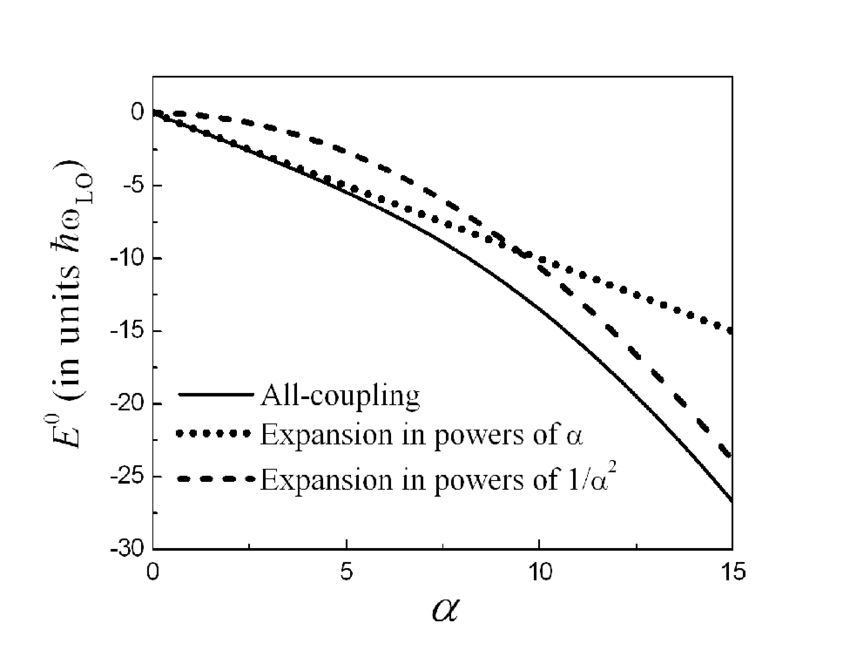
\includegraphics[scale=1.0]{Feynman-polaron-energy-as-a-function-of-a-the-all-coupling-theory.png}
    \caption{Computed polaron energy using perturbation theory, strong coupling theory and all coupling 
    Feynman technique \cite{article_coupling}.}
    \label{fig:coupling_strength_Froehlich}
\end{figure}
\subsection{Froehlich Hamiltonian with degenerate bands and multiple phonon modes}
The Hamiltonian in \ref{Froehlich_Hamiltonian_second} only describes an extremely limited number of real cases, namely a non-degenerate 
isotropic electron band with effective mass $m^*$ coupled to a single LO phonon mode. Although this relatively simple model is already 
quite challenging, some of its assumptions can be relaxed to obtain a more general framework.\\
Here we will be describing the \textbf{generalized Froehlich cubic model}: while mantaining some core simplification already seen in the 
original Froehlich model such as an isotropic dielectric tensor $\epsilon_0$ and $\epsilon_\infty$ together with a phonon dispersion $\omega_{jLO}$ which 
does not depend on the wavevector direction (an even more general model not restrained to the cubic case is described in \cite{miglio2020predominance}) $\hat{k}$, it is still a quite relevant and useful model since 
it can be used to describe multiple materials such as various oxides (BaO, CaO, MgO), II-VI compounds (CdS, CdSe, ZnS, ZnTe) and 
III-V compounds (AlAs, GaAs, GaN, GaP) \cite{guster2021frohlich}.
\begin{figure}[H]
    \centering
    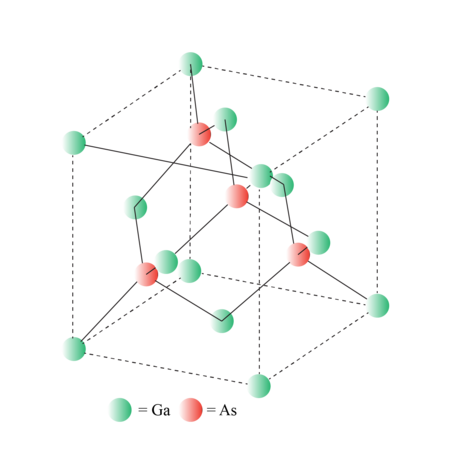
\includegraphics[scale=0.5]{GaAs_zincblende.png}
    \caption{GaAs crystal structure, the cubic structure of the zincblende unit cell is here clearly displayed.}
    \label{fig:GaAs_zincblende}
\end{figure}
We start by defining the new electron term:
\begin{equation}
    H^{cFr}_{el}\sum_{\mathbf{k}n}\frac{\sigma k^2}{2m^*_n(\hat{k})}c^\dagger_{\mathbf{k}n}c_{\mathbf{k}n},
    \label{cubic_froehlich_electron}
\end{equation}
where the sum has been extended to $n$ bands degenerate at the extremum, $\sigma=\pm 1$ depending on the fact that an electron or a hole 
polaron is taken into consideration, $m_n^*(\hat{k})$ is the new effective mass depending on band index $n$ and wavevector direction 
$\hat{k}$ (a tensorial quantity in general).\\
We also want to extend our Hamiltonian to tackle the case of multiple LO phonon modes present in the material, to this aim we define the 
following phonon term:
\begin{equation}
    H^{cFr}_{ph}=\sum_{\mathbf{q}j}\hbar\omega_{jLO}a^\dagger_{\mathbf{q}j}a_{\mathbf{q}j},
    \label{cubic_froehlich_phonon}
\end{equation}
where the index $j$ represents the different LO modes.\\
The electron-phonon coupling term gets redefined as:
\begin{equation}
    H^{cFr}_{EPC}=\sum_{\mathbf{k}nn',\mathbf{q}j}c^\dagger_{\mathbf{k}+\mathbf{q}n'}c_{\mathbf{k}n}\left[V^{cFr}(\mathbf{k}nn',\mathbf{q}j)a_{\mathbf{q}j}+V^{*cFr}(\mathbf{k}nn',\mathbf{q}j)a^\dagger_{-\mathbf{q}j}\right].
\end{equation}
It should be noted that the new electron-phonon coupling term includes interband transitions (from $n$ to $n'$). The new coupling strength 
$V^{cFr}(\mathbf{k}nn',\mathbf{q}j)$ is found to be
\begin{equation}
    V^{cFr}(\mathbf{k}nn',\mathbf{q}j)=\frac{i}{q}\frac{4\pi}{\Omega_0}\left(\frac{1}{2\omega_{jLO}V_{BvK}}\right)^{1/2}\frac{p_{jLO}}{\epsilon_\infty}\times \sum_{m}s_{n'm}(\hat{k}')s^*_{nm}(\hat{k}),
\end{equation}
with $\Omega_0$ volume of the primitive unit cell, $V_{BvK}$ volume of the Born-von Karman unit cell, $p_{jLO}$ phonon mode polarities, linked to Born 
effective charges and ionic dielectric tensor $\epsilon_0$ \cite{gonze1997dynamical} and computed as $p_{jLO}(\hat{q})=\sum_\nu Z^*_\nu e_\nu(\hat{q})$ isotropic in cubic 
system, and the $s$ tensors, symmetry dependent unitary matrices which represent specific bands (and have the same symmetry group).
\begin{figure}[H]
    \centering
    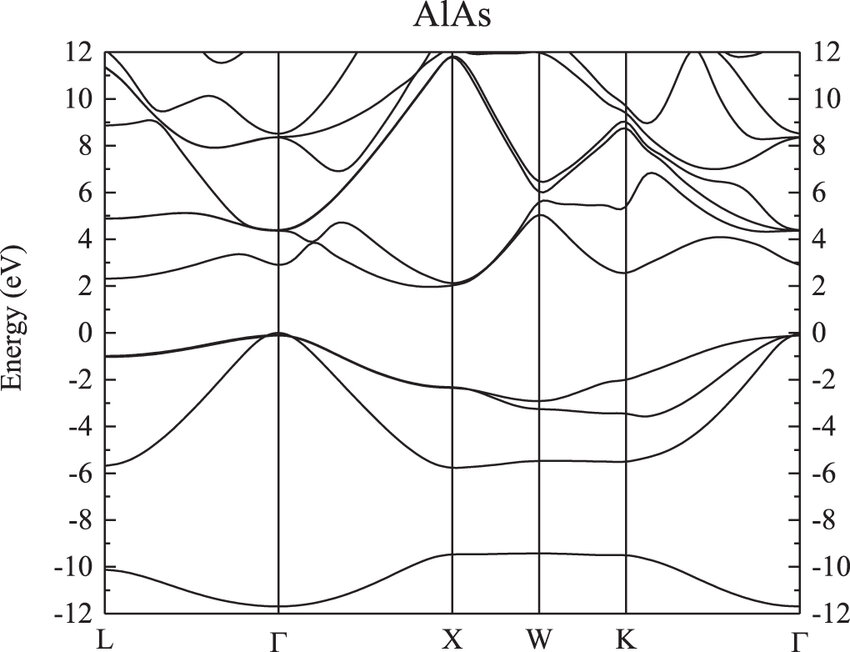
\includegraphics[scale=1.0]{Electronic-band-structure-for-AlAs.jpg}
    \caption{DFT calculated AlAs band structure \cite{da2021pseudopotential}, the conduction band minimum is on the high symmetry 
    line $\Delta$ between $\Gamma$ and $X$.}
    \label{fig:AlAs_bands}
\end{figure}
In our case of interest we restrict to just one anisotropic non-degenrate electron band, which is an accurate model for the conduction band minimum of 
the materials cited before (usually located somewhere between $\Gamma$ and $X$ along the $\Delta$ line), in this case the interaction 
strength simplifies to:
\begin{equation}
    V^{cFr}(qj)=\frac{i}{q}\frac{4\pi}{\Omega_0}\left(\frac{1}{2\omega_{jLO}V_{BvK}}\right)^{1/2}\frac{p_{jLO}}{\epsilon_\infty},
    \label{coupling_strength_anisotropic}
\end{equation}
and the full Hamiltonian reads:
\begin{equation}
    H^{cFr}=\sum_{\mathbf{k}}\frac{\sigma k^2}{2m^*(\hat{k})}c^\dagger_\mathbf{k}c_\mathbf{k}+\sum_{\mathbf{q}j}\hbar\omega_{jLO}a^\dagger_{\mathbf{q}j}a_{\mathbf{q}j}+\sum_{\mathbf{k},\mathbf{q}j}c^\dagger_{\mathbf{k}+\mathbf{q}}c_\mathbf{k}\left[V^{cFr}(qj)a_\mathbf{q}+V^{*cFr}(qj)a^\dagger_\mathbf{-q}\right].
    \label{Froehlich_cubic_k_anisotropic}
\end{equation}
The effective mass $m^*(\hat{k})$ dependence on the wavevector $\mathbf{q}$ direction is expressed in the following way:
\begin{equation}
    \frac{1}{m^*(\hat{k})}=\frac{\hat{k}_x^2}{m^*_x}+\frac{\hat{k}_y^2}{m^*_y}+\frac{\hat{k}_z^2}{m^*_z},
    \label{effective_mass_anisotropic_relation}
\end{equation}
with $m^*_x$, $m^*_y$ and $m^*_z$ effective mass values on the three cartesian axes.\\
Alternatively, the following formula for the electron energy as a function of $k$ can be employed:
\begin{equation}
    \epsilon(\mathbf{k})=\frac{\sigma}{2}\left(\frac{k^2_x}{m^*_x}+\frac{k_y^2}{m^*_y}+\frac{k_z^2}{m^*_z}\right).
\end{equation}
\section{The Froehlich polaron: Feynman diagrams}
In order to deeply understand a many-body system such as the Froehlich polaron it is necessary to use a more powerful formalism 
derived from quantum field theory, we will first breafly describe Green's functions as an effective mean to describe meaningful quantities of 
our system and we will then shift to the \textbf{Matsubara imaginary time} formalism, much more useful in the context of Diagrammatic Monte Carlo.
At the end of this journey the connection between the Froehlich polaron and Feynman diagrams will be explicated. In this section of the thesis 
we will use the convention $\hbar=1$.
\subsection{Green's function formalism}
Green functions are useful objects to perturbatively solve systems that are really hard to correctly treat in any other way \cite{bruus2004many}.\\
If we take for example a time-dependent Schroedinger equation in the following way:
\begin{equation}
    \left[i\partial_t - H_0(\mathbf{r})-V(\mathbf{r})\right]\psi(\mathbf{r},t)=0,
    \label{Schroedinger_eq_hamiltonian}
\end{equation}
with the non-interacting diagonizable term $H_0$ and the perturbation $V$. It is possible to define the corresponding Green's functions as:
\begin{equation}
\begin{split}
    \left[i\partial_t -H_0(\mathbf{r})\right]G_0(\mathbf{r},\mathbf{r}';t,t')&=\delta(\mathbf{r}-\mathbf{r}')\delta(t-t'),\\
    \left[i\partial_t -H_0(\mathbf{r})-V(\mathbf{r})\right]G(\mathbf{r},\mathbf{r}';t,t')&=\delta(\mathbf{r}-\mathbf{r}')\delta(t-t').
\end{split}
    %\left[E-H_0(\mathbf{r})\right]G_0(\mathbf{r},\mathbf{r}',E)=\delta(\mathbf{r}-\mathbf{r'}),\hspace{0.5cm}with\hspace{0.5cm}G_0(\mathbf{r},\mathbf{r}')=G_0(\mathbf{r}',\mathbf{r}).
\end{equation}
We can define $G_0^{-1}(\mathbf{r};t')$ and $G^{-1}(\mathbf{r};t)$ as:
\begin{equation}
\begin{split}
    &G_0^{-1}(\mathbf{r};t)=i\partial_t-H_0(\mathbf{r}),\\
    &G^{-1}(\mathbf{r};t)=i\partial_t-H_0(\mathbf{r})-V(\mathbf{r}),
\end{split}
\label{GF_solving_eq}
\end{equation}
%and thus
%\begin{equation}
%    G_0^{-1}(\mathbf{r},E)G_0(\mathbf{r},\mathbf{r}',E)=\delta(\mathbf{r},\mathbf{r}').
%\end{equation}
The Schroedinger equation can then be recast as
\begin{equation}
    \left[G^{-1}_0(\mathbf{r},t)-V(\mathbf{r})\right]\psi(\mathbf{r},t)=0
\end{equation}
and it is possible to rewrite the system as an integral equation
\begin{equation}
    \psi(\mathbf{r},t)=\psi^0(\mathbf{r},t)+\int d^3r'\int dt' G_0(\mathbf{r},\mathbf{r}';t,t')V(\mathbf{r}')\psi(\mathbf{r}',t')
    \label{GF_expansion_integral}
\end{equation}
which can be solved iteratively. In fact:
\begin{equation}
\begin{split}
    %\psi_E(\mathbf{r})=\psi^0_E(\mathbf{r})+\int d^3 r'G_0(\mathbf{r},\mathbf{r}',E)V(\mathbf{r}')\psi_E^0(\mathbf{r}')+O(V^2).
    \psi&= \psi^0+G_0V\psi^0+G_0VG_0V\psi^0+G_0VG_0VG_0V\psi^0+...\\
    &= \psi^0+(G_0+G_0VG_0+G_0VG_0VG_0+...)V\psi_0.
\end{split}
\label{expansion_G}
\end{equation}
Noting that \ref{GF_expansion_integral} can be also written as:
\begin{equation}
    \psi(\mathbf{r},t)=\psi^0(\mathbf{r},t)+\int d^3r'\int dt' G(\mathbf{r},\mathbf{r}';t,t')V(\mathbf{r}')\psi^0(\mathbf{r}',t'),
\end{equation}
it is possible to identify $G$ with
\begin{equation}
\begin{split}
    G&=G_0+G_0VG_0+G_0VG_0VG_0+...\\
    &=G_0+G_0V(G_0+G_0VG_0+...),
\end{split}
\end{equation}
and the well-known \textbf{Dyson equation} is retrieved:
\begin{equation}
    G=G_0+G_0VG.
    \label{Dyson_Eq}
\end{equation}
The one described above is the \textbf{single particle Green's function}, also called propagator since it "propagates" the wavefunction: in fact,
if the wavefunction is known at time $t'$ the wavefunction at a later time can be obtained in the following way:
\begin{equation}
    \psi(\mathbf{r},t)=\int d^3r'\int dt' G(\mathbf{r}t,\mathbf{r}'t')\psi(\mathbf{r}'t'),
\end{equation}
which is a solution to \ref{GF_solving_eq}.
The Green's function can also be written as
\begin{equation}
    G(\mathbf{r}t,\mathbf{r}'t')=-\theta(t-t')\langle \mathbf{r}|e^{-iH(t-t')}|\mathbf{r}'\rangle,
\end{equation}
and is more precisely known as the \textbf{retarded Green's function}.\\
Focusing now on a many-body system the Green's function is defined as
\begin{equation}
    G^R(\mathbf{r}\sigma t,\mathbf{r}'\sigma't')=-i\theta(t-t')\langle[\psi_\sigma(\mathbf{r},t),\psi^\dagger_{\sigma'}(\mathbf{r}',t')]_{B,F}\rangle,
\end{equation}
where $[,]_{B,F}$ is the commutator $[,]$ for bosons and the anticommutator $\{,\}$ for fermions.\\
In the case of translation-invariant system (such as lattices) Green's functions can only depend on $\mathbf{r}-\mathbf{r}'$ and 
it is natural to adopt the usual $\mathbf{k}$ formalism:
\begin{equation}
\begin{split}
    G^R(\mathbf{r}-\mathbf{r}',\sigma t,\sigma' t')&=\frac{1}{V}\sum_\mathbf{k}e^{i\mathbf{k}\cdot(\mathbf{r}-\mathbf{r}')}G^R(\mathbf{k},\sigma t,\sigma' t'),\\
    G^R(\mathbf{k},\sigma t,\sigma' t')&=-i\theta (t-t')\langle [a_{\mathbf{k}\sigma},a^\dagger_{\mathbf{k}'\sigma'}]_{B,F}\rangle.
\end{split}
    \label{GF_momentum_space}
\end{equation}
The goal is now to find explicit expressions for the various Green's function of relevance, in the special case of a free electron 
the Hamiltonian assumes the simple form
\begin{equation}
    H=\sum_{\mathbf{k}\sigma}\epsilon(k)c^\dagger_{\mathbf{k}\sigma}c_{\mathbf{k}\sigma},
\end{equation}
and the time dependence of the creation/annihilation operators is simply defined as
\begin{equation}
    c_{\mathbf{k}\sigma}(t)=e^{iHt}c_{\mathbf{k}\sigma}e^{-iHt}=c_{\mathbf{k}\sigma}e^{-i\xi_kt}.
\end{equation}
The retarded Green's function then becomes:
\begin{equation}
    G^R(\mathbf{k}\sigma,t-t')=-i\theta(t-t')e^{-i\xi_k(t-t')}.
\end{equation}
\subsection{Matsubara formalism for imaginary time Green's functions}
The usual Green's functions are complex objects that are not fit to be used in the Diagrammatic Monte Carlo method since they provides 
negative values that cannot be easily sampled from a distribution without losing precision.\\
For this reason we now describe the imaginary time formalism for Green's functions, which is also useful to evaluate system that are 
at non-zero temperature. The relevant substitution is:
\begin{equation}
    it\to \tau,
    \label{imaginary_time_substitution}
\end{equation}
%it is important to stress that this imaginary time formalism does not have any physical meaning and is just an useful mathematical framework.\\
the retarded Green's function previously defined in \ref{GF_momentum_space} thus becomes:
\begin{equation}
    G^R(\mathbf{k},\sigma\tau,\sigma'\tau')=-\theta(\tau-\tau')\langle [a_{\mathbf{k}\sigma},a^\dagger_{\mathbf{k}'\sigma'}]_{B,F}\rangle
\end{equation}
where the thermal average $\langle A(\tau)B(\tau')\rangle$ is defined as:
\begin{equation}
\begin{split}
    &\langle \Psi_0|A(\tau)B(\tau')|\Psi_0\rangle\hspace{1.75cm}T=0,\\
    &\frac{1}{Z}Tr\left[e^{-\beta H}A(\tau)B(\tau')\right]\hspace{0.8cm}T>0.
\end{split}
\end{equation}
where $\Psi_0$ is the ground state and $Z$ the partition function.\\
Given a system with a Hamiltonian characterized by a diagonizable term $H_0$ and a perturbation $V(\tau)$, we can define the imaginary time 
Heisenberg picture for an operator $A$ as 
\begin{equation}
    A(\tau)=e^{-\tau H}Ae^{\tau H},
\end{equation}
and similarly the imaginary time interaction picture as
\begin{equation}
    A_I(\tau)=e^{\tau H_0}Ae^{-\tau H_0}.
\end{equation}
We can define the imaginary time time-evolution operator in the interaction picture as 
\begin{equation}
    U_I(\tau,\tau')=e^{\tau H_0}e^{-(\tau-\tau')H}e^{-\tau'H_0},
\end{equation}
an explicit expression for the interaction picture time-evolution operator in the imaginary time formalism is found in analogy with 
the real time counterpart
\begin{equation}
    \partial_\tau U_I(\tau,\tau')=e^{\tau H_0}(H_0-H)e^{-(\tau-\tau')H}e^{-\tau'H_0}=-V_I(\tau)U_I(\tau,\tau'),
\end{equation}
which can be solved iteratively:
\begin{equation}
\begin{split}
    U_I(\tau,\tau')&=\sum_{n=0}^\infty\frac{1}{n!}(-1)^n\int_{\tau'}^{\tau}d\tau_1...\int{\tau'}^{\tau}d\tau_nT_\tau\left[V_I(\tau_1)...V_I(\tau_n)\right]\\
    &=T_\tau\exp{\left(-\int_{\tau'}^\tau d\tau_1V_I(\tau_1)\right)},
\end{split}
\end{equation}
where $T_\tau$ is the $\tau$ ordering operator.\\
It is also important to stress that the partition function $Z$ is naturally treated in the imaginary time formalism, in fact:
\begin{equation}
    e^{-\beta H}=e^{-\beta H_0}U_I(\beta,0)=e^{-\beta H_0}T_\tau exp{\left(-\int_{0}^{\beta}d\tau_1V_I(\tau_1)\right)},
\end{equation}
and we have
\begin{equation}
\begin{split}
    \langle T_\tau A(\tau)B(\tau')\rangle &= \frac{1}{Z}Tr\left[e^{-\beta H}T_\tau(A(\tau)B(\tau'))\right]\\
    &=\frac{1}{Z}Tr\left[e^{-\beta H_0}U_I(\beta,0)T_\tau(U_I(0,\tau)A_I(\tau)U_I(\tau,\tau')B_I(\tau')U_I(\tau',0)) \right]\\
    &=\frac{1}{Z}Tr\left[e^{-\beta H_0}T_\tau(U_I(\beta,0)A_I(\tau)B_I(\tau'))\right]\\
    &=\frac{\langle T_\tau U_I(\beta,0)A_I(\tau)B_I(\tau')\rangle_0}{\langle U_I(\beta,0)\rangle_0}.
\end{split}
\end{equation}
We now go back to the definition of single particle Green's functions in imaginary time formalism, we can define them both in real space 
and in $\mathbf{k}$ space:
\begin{equation}
\begin{split}
    &G(\mathbf{r}t,\mathbf{r}'t')=-\langle T_\tau\left(\psi(\mathbf{r},\tau),\psi^\dagger(\mathbf{r}',\tau')\right)\rangle,\\
    &G(\mathbf{k}\tau,\mathbf{k}'\tau')=-\langle T_\tau\left(c_{\mathbf{k}}(\tau)c^\dagger_{\mathbf{k}'}(\tau')\right)\rangle,
\end{split}
\end{equation}
neglecting the spin $\sigma$ degree of freedom (not relevant for our treatment).\\
In the non-interacting case the Matsubara single particle Green's functions can be valued in the same way as the retarded Green's functions, 
in fact:
\begin{equation}
    H_0=\sum_{\mathbf{k}}\xi_\mathbf{k}c^\dagger_\mathbf{k}c_\mathbf{k},
\end{equation}
and the creation/annihilation operators in the Heisenberg picture read
\begin{equation}
    c_\mathbf{k}(\tau)=e^{\tau H_0}c_\mathbf{k}e^{-\tau H_0}=c_\mathbf{k}e^{-\xi_\mathbf{k}\tau},\hspace{1cm}c^\dagger_\mathbf{k}(\tau)=e^{\tau H_0}c^\dagger_\mathbf{k}e^{-\tau H_0}=c^\dagger_\mathbf{k}e^{\xi_\mathbf{k}\tau}.
\end{equation}
The non-interacting Matsubara Green's function is then defined as 
\begin{equation}
\begin{split}
    G_0(\mathbf{k},\tau,\tau')&=-\langle T_\tau\left(c_\mathbf{k}(\tau)c^\dagger_\mathbf{k}(\tau')\right)\rangle\\
    &=-\theta(\tau-\tau')\langle c_\mathbf{k}(\tau)c^\dagger_\mathbf{k}(\tau')\rangle-(\pm)_{B,F}\theta(\tau'-\tau)\langle c^\dagger_\mathbf{k}(\tau')c_\mathbf{k}(\tau)\rangle\\
    &=-\left[\theta(\tau-\tau')\langle c_\mathbf{k}c^\dagger_\mathbf{k}\rangle-(\pm)_{B,F}\theta(\tau'-\tau)\langle c_\mathbf{k}^\dagger c_\mathbf{k}\rangle\right]e^{-\xi_\mathbf{k}(\tau-\tau')}.
    \label{free_propagator}
\end{split}
\end{equation}
We may now consider the Froehlich Hamiltonian previously defined in \ref{Froehlich_cubic_k_anisotropic} using the new imaginary time formalism,
defining the non-interacting Hamiltonian $H^{cFr}_0$ as 
\begin{equation}
    H^{cFr}_0=\sum_\mathbf{k}\frac{\sigma k^2}{2m(\hat{k})}c^\dagger_{\mathbf{k}}c_\mathbf{k}+\sum_{\mathbf{q}j}\omega_{LO}a^\dagger_{\mathbf{q}j}a_{\mathbf{q}j}.
    \label{polaron_non-interacting}
\end{equation}
Since our model consists of a single electron (hole) in the minimum (maximum) of the conduction (valence) band interacting with a cloud of phonon, we may 
consider our system to be at zero temperature and the ground state wavefunction $|\Psi_0\rangle$ to be the vacuum:
\begin{equation}
    |\Psi_0\rangle=|0\rangle,\hspace{1cm}\langle \cdot \rangle=\langle 0|\cdot|0\rangle
\end{equation}
It is then possible to explicitely compute the electron free propagator using \ref{free_propagator}:
\begin{equation}
\begin{split}
    G_0(\mathbf{k},\tau,\tau')&=-\left[\theta(\tau-\tau')\langle 0| c_\mathbf{k}c^\dagger_\mathbf{k}|0\rangle+\theta(\tau'-\tau)\langle 0 | c^\dagger_\mathbf{k}c_\mathbf{k}|0\rangle\right]e^{k^2/2m(\hat{k})(\tau-\tau')}\\
    &=-\theta(\tau-\tau')e^{(k^2/2m(\hat{k}))(\tau-\tau')},
\end{split}
\end{equation}
which for $\tau'=0$ becomes
\begin{equation}
    G_0(\mathbf{k},\tau)=-e^{(k^2/2m(\hat{k}))\tau},\hspace{1cm}\tau\ge0.
\end{equation}
The Matsubara Green function for a free electron propagator assumes the simple form of an exponential function, which can be easily sampled.\\
In the same way, it is possible to find an explicit form for the phonon free propagator:
\begin{equation}
    D_0(\mathbf{q}j,\tau)=-e^{\omega_{jLO}\tau},\hspace{1cm}\tau\ge0,
\end{equation}
which is again a simple exponential function.
\printbibliography
\end{document}